\documentclass{beamer}
% There are many different themes available for Beamer. A comprehensive
% list with examples is given here:
% http://deic.uab.es/~iblanes/beamer_gallery/index_by_theme.html
% You can uncomment the themes below if you would like to use a different
% one:
%%\usetheme{AnnArbor}
\usetheme{Antibes}
%\usetheme{Bergen}
%\usetheme{Berkeley}
%\usetheme{Berlin}
%\usetheme{Boadilla}
%\usetheme{Frankfurt}
%\usetheme{boxes}
%\usetheme{CambridgeUS}
%\usetheme{Copenhagen}
%\usetheme{Darmstadt}
%\usetheme{focus}
\usepackage{hologo}

\usepackage{tikz}
\usepackage{url}
\usepackage{color}
\usepackage{longtable}
\usepackage{booktabs}
\usetikzlibrary{shapes.geometric, arrows, positioning, calc}
\tikzstyle{startStop} = [rectangle, rounded corners, minimum width=7cm, text width=11cm, text centered, minimum height=.5cm, draw=black]
\tikzstyle{io} = [circle, rounded corners, minimum width=1cm, text width=1.5cm, minimum height=.1, text centered, draw=black]
\tikzstyle{arrow} = [thick,->,>=stealth]
\usepackage{pdfpages}
\usepackage{graphicx}   % need for figures
\usepackage{adjustbox}
\usepackage{fontawesome}
\usepackage[absolute,overlay]{textpos}
%CHANGES COLOR TO GREEN
\usepackage{listings}
\usepackage{color}
% for game design diagram
\usetikzlibrary{trees}

\usepackage{verbatim}

\definecolor{codegreen}{rgb}{0,0.6,0}
\definecolor{codegray}{rgb}{0.5,0.5,0.5}
\definecolor{codepurple}{rgb}{0.58,0,0.82}
\definecolor{backcolour}{rgb}{0.95,0.95,0.92}

\lstdefinestyle{mystyle}{
	backgroundcolor=\color{backcolour},
	commentstyle=\color{codegreen},
	keywordstyle=\color{magenta},
	numberstyle=\tiny\color{codegray},
	stringstyle=\color{codepurple},
	basicstyle=\scriptsize,
	breakatwhitespace=true,
	breaklines=true,
	captionpos=b,
	keepspaces=false,
	numbers=left,
	numbersep=5pt,
	showspaces=false,
	showstringspaces=false,
	showtabs=false,
	tabsize=2
}
\hypersetup{
	colorlinks = true,
	linkcolor=brickred,   % color of internal links
	citecolor=brickred,   % color of links to bibliography
	urlcolor=brickred,    % color of external links
	%	pagebackref=true,
	%	implicit=false,
	%	bookmarks=true,
	bookmarksopen=true,
	pdfdisplaydoctitle=true
}
\lstset{style=mystyle}
\definecolor{brickred}{rgb}{0.8, 0.25, 0.33}
\definecolor{mygreen}{cmyk}{0.82,0.11,1,0.25}
\setbeamertemplate{blocks}[rounded][shadow=false]
\addtobeamertemplate{block begin}{\pgfsetfillopacity{0.8}}{\pgfsetfillopacity{1}}
\setbeamercolor{structure}{fg=mygreen}
\setbeamercolor*{block title example}{fg=white,
	bg= white}
\setbeamercolor*{block body example}{fg= white,
	bg= white}
\usepackage[english]{babel}
\usepackage{hyperref}
\usepackage{dcolumn}
\usepackage{adjustbox}
\usepackage{multicol}
\usepackage{adjustbox}
\usepackage{amsmath}
\usepackage{tikz}
\usepackage[all,cmtip]{xy}
\tikzstyle{largeSquare} = [rectangle, rounded corners, minimum width=7cm, text width=9cm, minimum height=.5cm, draw=black]
\usepackage{tikzsymbols}

\usetikzlibrary{shapes.geometric, arrows}
\tikzstyle{arrow}=[thick,->,>=stealth]
\beamertemplatenavigationsymbolsempty
\usepackage{subfloat}
\setbeamertemplate{headline}{}
\newcommand{\speechthis}[2]{
	\tikz[remember picture,baseline]{\node[anchor=base,inner sep=0,outer sep=0]
		(#1) {\underline{#1}};\node[overlay,ellipse callout,fill=blue!50]
		at ($(#1.north)+(-.5cm,0.8cm)$) {#2};}
}

\setbeamercolor{button}{bg=mygreen,fg=white}

\setbeamercovered{invisible}

\usecolortheme{beaver} %TODO

\definecolor{codegreen}{rgb}{0,0.6,0}
\definecolor{codegray}{rgb}{0.5,0.5,0.5}
\definecolor{codepurple}{rgb}{0.58,0,0.82}
\definecolor{backcolour}{rgb}{0.95,0.95,0.92}

\lstdefinestyle{mystyle}{
	backgroundcolor=\color{backcolour},
	commentstyle=\color{codegreen},
	keywordstyle=\color{magenta},
	numberstyle=\tiny\color{codegray},
	stringstyle=\color{codepurple},
	basicstyle=\footnotesize,
	breakatwhitespace=false,
	breaklines=true,
	captionpos=b,
	keepspaces=true,
	numbers=left,
	numbersep=5pt,
	showspaces=false,
	showstringspaces=false,
	showtabs=false,
	tabsize=2
}
\lstset{style=mystyle}
\newcommand{\Sref}[1]{Section~\ref{#1}}
\newtheorem{hyp}{Hypothesis}

\title{Choice and Personal responsibility\\What is a morally relevant choice?}
\author{Imelda Finn}
\subtitle{Applied Statistical Analysis II}
\date{Spring 2023}
\begin{document}
	\frame{\titlepage}

	\begin{frame}{Background/introduction}

		\begin{block}

			\begin{itemize}

				\item Introduction \vspace{.25cm}
				\begin{itemize}
					\item Alexander W. Cappelen, Sebastian Fest, Erik Ø. Sørensen, Bertil Tungodden
					\item September 12, 2018
					\item Norwegian School of Economics, Bergen, Norway
					\item \href{https://dataverse.harvard.edu/dataset.xhtml?persistentId=doi:10.7910/DVN/A6KFNO}{Data from Harvard Dataverse, FAIR - Centre for Experimental Research on Fairness, Inequality and Rationality}
					\item 					\url{https://cee.boun.edu.tr/sites/cee.boun.edu.tr/files/documents/CEE2018Conference/cprwmrc.pdf} %cite
				\end{itemize}
			\end{itemize}
		\end{block}
	\end{frame}

	\begin{frame}{Theory}

	\begin{block}

		\begin{itemize}
			\item Inequality is tolerated because people are blamed for their choices/outcomes.
			\item A person should \textbf{not} be held personally responsible for the outcome of a choice if:
			\begin{itemize}
				\item the person could not have changed the likelihood of the outcome by choosing differently 	(\textbf{no ex ante causal responsibility}), or
				\item  the person could only have avoided the outcome at unreasonably large cost (\textbf{no acceptable alternative}).
			\end{itemize}
			\item 	$H_0$ a trivial choice will make no difference to the outcome.
		\end{itemize}
	\end{block}
\end{frame}

%------------------------------------------------------------------------------------
	\begin{frame}{Game Design}
		%\documentclass{article}

%\usepackage[latin1]{inputenc}
%\usepackage{tikz}
%\usetikzlibrary{trees}
%\begin{document}
%\thispagestyle{empty}

% Set the overall layout of the tree
\tikzstyle{level 1}=[level distance=1.5cm, sibling distance=3.75cm]
\tikzstyle{level 2}=[level distance=1.75cm, sibling distance=2.25cm]
\tikzstyle{level 3}=[level distance=2.0cm, sibling distance=2.0cm]

% Define styles for bags and leafs
\tikzstyle{bag} = [text width=4.0em, text centered]
\tikzstyle{end} = [circle, minimum width=2.5pt,fill, inner sep=0pt]

% The sloped option gives rotated edge labels. Personally
% I find sloped labels a bit difficult to read. Remove the sloped options
% to get horizontal labels. 
\begin{figure}
\begin{tikzpicture}[sloped] %grow=right,
\node[bag] {\normalsize Game Tree}
  child{
    node[bag] {\small Base }
    child {
        node[bag] {\small Nature}        
            child {
                node[end, label=left:{\small L}] {}
                edge from parent
                node[above] {\scriptsize yellow}
                node[below] {\scriptsize $p=0.5$}
            }
            child {
                node[end, label=left:{\small 0}] {}
                edge from parent
                node[above] {\scriptsize green}
                node[below] {\scriptsize $p=0.5$}
            }
            edge from parent 
%            node[above] {lottery}
    }
  }
  child{
    node[bag] {\small Nominal Choice \\Participant}
    child {
        node[bag] {\small Nature}        
            child {
                node[end, label=left:{\small L}] {}
                edge from parent
                node[above] {\scriptsize yellow}
                node[below] {\scriptsize $p=0.5$}
            }
            child {
                node[end, label=left:{\small 0}] {}
                edge from parent
                node[above] {\scriptsize green}
                node[below] {\scriptsize $p=0.5$}
            }
            edge from parent 
            node[above] {\scriptsize yellow}
    }
    child {
        node[bag] {\small Nature}        
            child {
                node[end, label=right:{\small L}] {}
                edge from parent
                node[above] {\scriptsize yellow}
                node[below] {\scriptsize $p=0.5$}
            }
            child {
                node[end, label=left:{\small 0}] {}
                edge from parent
                node[above] {\scriptsize green}
                node[below] {\scriptsize $p=0.5$}
            }
            edge from parent 
            node[above] {\scriptsize green}
    }
  }
  child{
    node[bag] {\small Forced Choice \\Participant}
    child {
		node[end,label=left:{\small S}] {}      
		edge from parent 
		node[above] {\scriptsize safe}
	}
    child {
        node[bag] {\small Nature}        
            child {
                node[end, label=left:{\small L}] {}
                edge from parent
                node[above] {\scriptsize yellow}
                node[below] {\scriptsize $p=0.5$}
            }
            child {
                node[end, label=left:{\small 0}] {}
                edge from parent
                node[above] {\scriptsize green}
                node[below] {\scriptsize $p=0.5$}
            }
            edge from parent 
            node[above] {\scriptsize lottery}
    }
  }
  ;
\end{tikzpicture}
\caption{\footnotesize Note: The figure shows the sequential form game representation of how the earnings were determined in each of the three treatments
in the experiments.\tiny Lab: L = 800,S = 25 (NOK); Online: L = 8, S$\in (-0.25, 0, 0.25)$ (USD)}%

\label{fig:gametree}
\end{figure}

%\end{document}
%		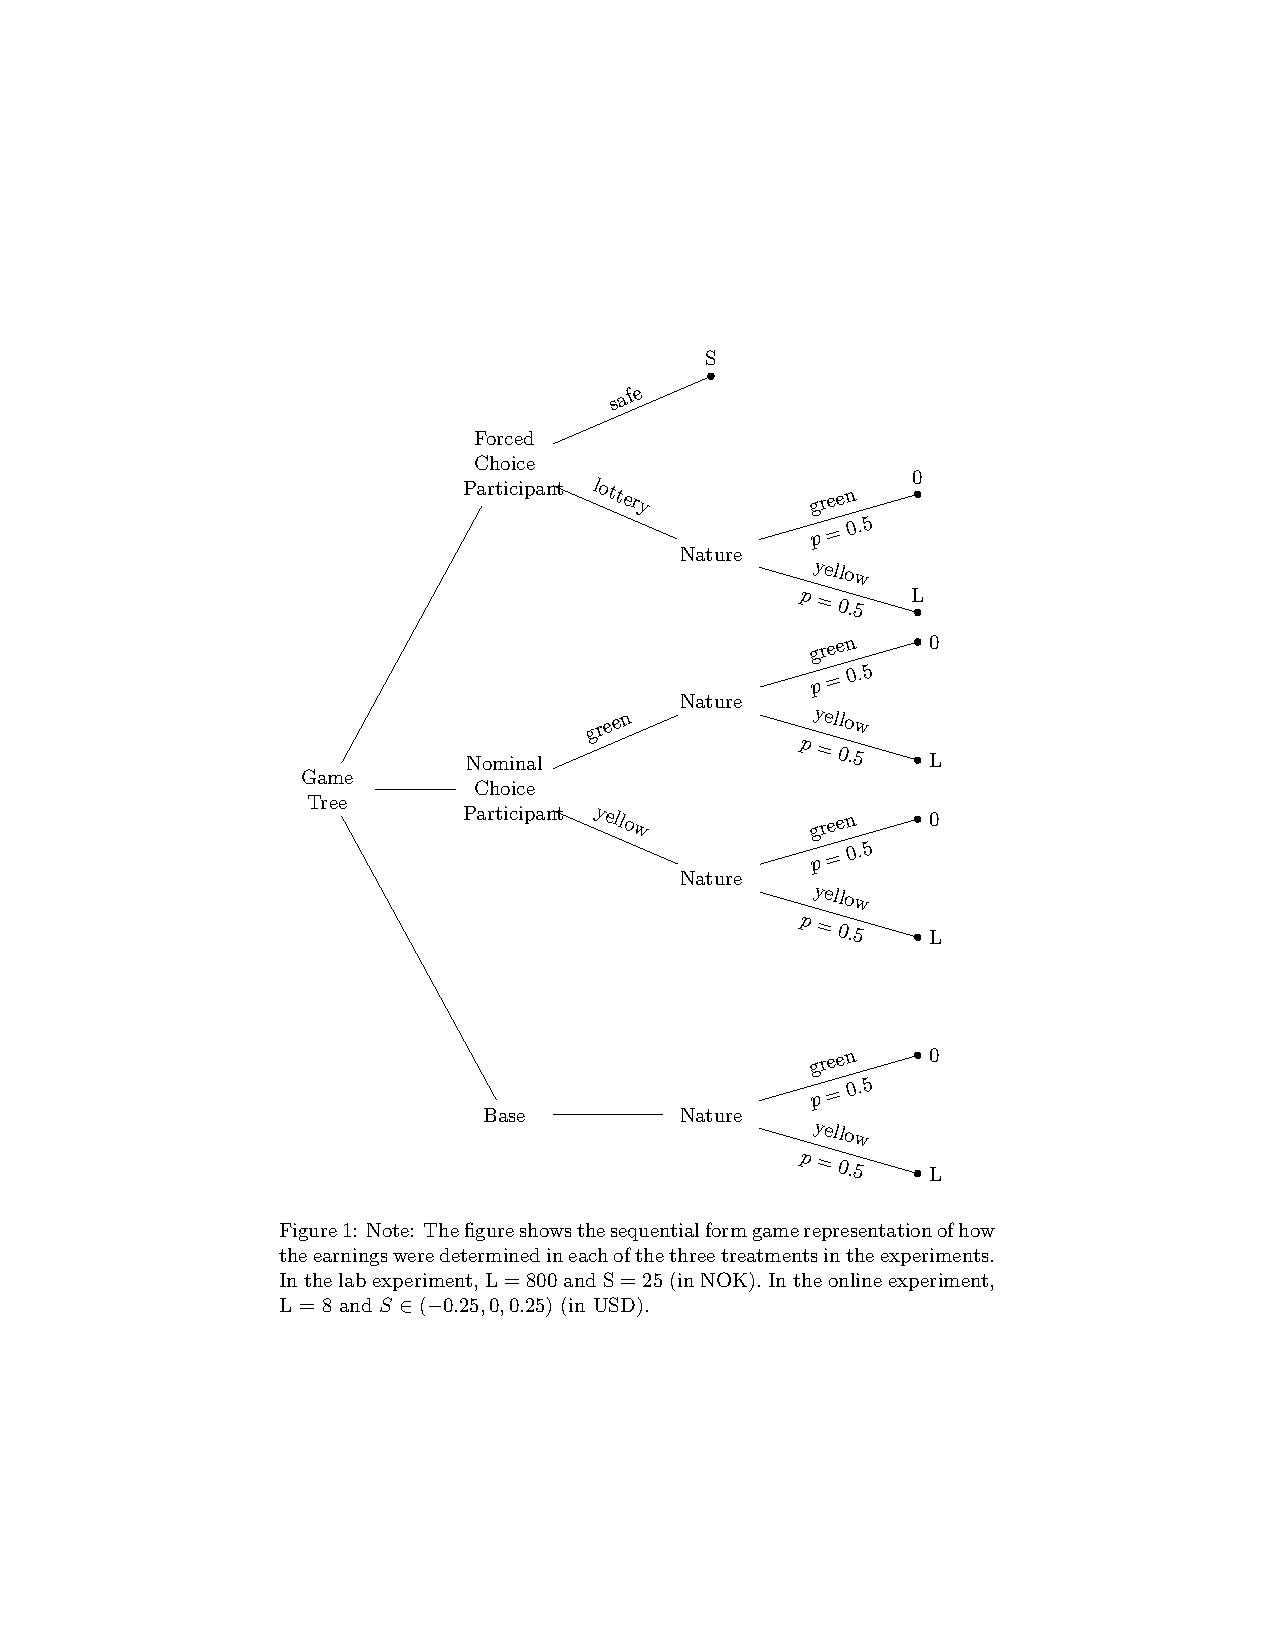
\includegraphics[width=.75\textwidth]{moral_tree.pdf}
	\end{frame}
%------------------------------------------------------------------------------------

	\begin{frame}{Experimental Design}

	\begin{block}

		\begin{itemize}
			\item Studying spectators decision to redistribute money/not
			\item payment allocated in all cases by lottery - picking green/yellow ball.
			\item random allocation to treatment, no interaction - blind trial
			\item background information about age, gender, and political affiliation
			\item three-item cognitive reflection test measuring the ability to correct for incorrect
				intuitive answers through reflection.
		\end{itemize}
	\end{block}
\end{frame}

%------------------------------------------------------------------------------------
	\begin{frame}{Lab Experiment}

	\begin{block}

		\begin{itemize}
			\item 422 participants from 2 Norwegian colleges
			\item average age 22.7 years, 54\% male, average CRT score 1.6/3, 41\% self-reported support for a right-wing party in Norway\footnote{close to the distribution of votes in the last election in Norway.}
			\item 800 NOK or 0
			\item all worked at simple task
			\item  spectators were participants; they didn't know when making choice if they had gotten money
			\item spectators asked what motivated their decision to redistribute/not.
			\item Average payment was 475 NOK (approximately 80 USD) incl 100 basic fee.
		\end{itemize}
	\end{block}
\end{frame}

%------------------------------------------------------------------------------------

  	\begin{frame}{Lab Experiment Transfers}
		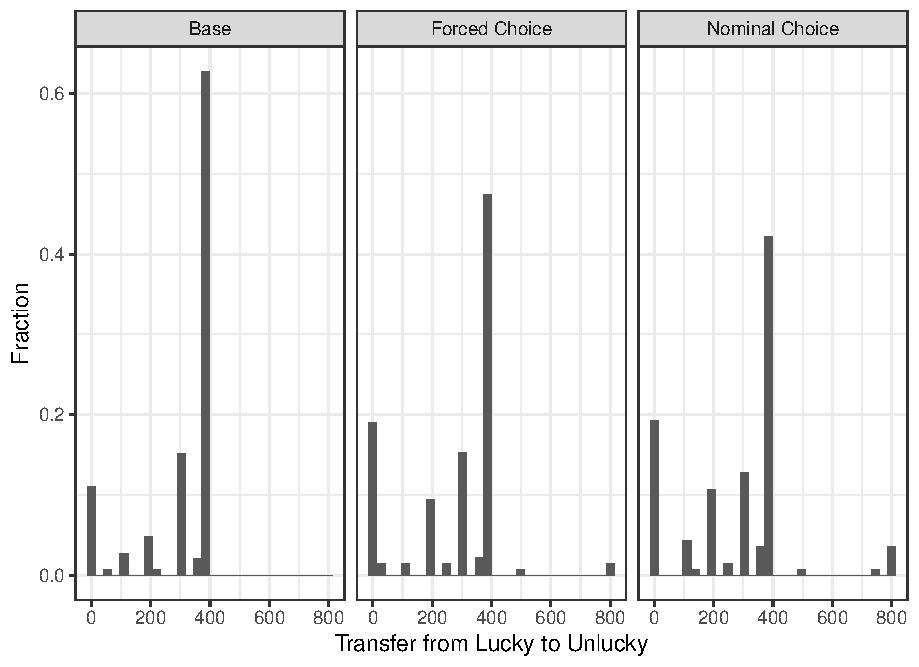
\includegraphics[height=.9\textheight]{../graphs/histograms_lab.pdf}
	\end{frame}
%------------------------------------------------------------------------------------
\begin{frame}{Lab Experiment Inequality}
	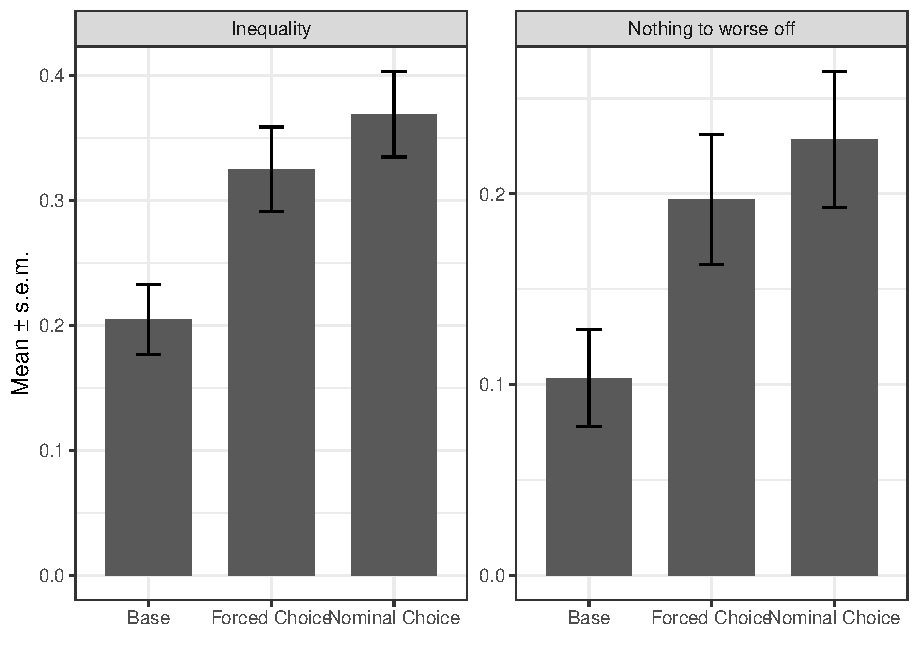
\includegraphics[height=.9\textheight]{../graphs/mean_ineq_nothing_lab.pdf}
	Note: The left panel shows the average inequality implemented by the spectators in each
	treatment, the right panel shows the share of spectators assigning no income to one of the
	participants in the pair in each of the treatments. The standard errors of the mean are indicated.
\end{frame}
%------------------------------------------------------------------------------------
		\begin{frame}{Table 1: Lab Results Regression 1: the role of choice}{\tiny
		%TODO still too long
		% Table created by stargazer v.5.2.3 by Marek Hlavac, Social Policy Institute. E-mail: marek.hlavac at gmail.com
		% Date and time: Fri, Mar 31, 2023 - 18:10:09

% Table created by stargazer v.5.2.3 by Marek Hlavac, Social Policy Institute. E-mail: marek.hlavac at gmail.com
% Date and time: Sat, Apr 01, 2023 - 00:21:19
\begin{table}[!htbp] \centering 
  \caption{} 
  \label{tbl:l1} 
\begin{tabular}{@{\extracolsep{5pt}}lcccc} 
\\[-1.8ex]\hline 
\hline \\[-1.8ex] 
\\[-1.8ex] & \multicolumn{2}{c}{inequality} & \multicolumn{2}{c}{zero\_to\_worst\_off} \\ 
\\[-1.8ex] & (1) & (2) & (3) & (4)\\ 
\hline \\[-1.8ex] 
 treatmentForced Choice & 0.120 & 0.125 & 0.094 & 0.101 \\ 
  & (0.044) & (0.044) & (0.043) & (0.042) \\ 
  & p = 0.007 & p = 0.005 & p = 0.028 & p = 0.017 \\ 
  & & & & \\ 
 treatmentNominal Choice & 0.164 & 0.163 & 0.125 & 0.128 \\ 
  & (0.044) & (0.044) & (0.044) & (0.043) \\ 
  & p = 0.001 & p = 0.001 & p = 0.005 & p = 0.003 \\ 
  & & & & \\ 
 leftp &  & $-$0.115 &  & $-$0.075 \\ 
  &  & (0.037) &  & (0.037) \\ 
  &  & p = 0.003 &  & p = 0.044 \\ 
  & & & & \\ 
 female &  & $-$0.108 &  & $-$0.159 \\ 
  &  & (0.040) &  & (0.039) \\ 
  &  & p = 0.007 &  & p = 0.000 \\ 
  & & & & \\ 
 age\_h &  & 0.017 &  & 0.051 \\ 
  &  & (0.037) &  & (0.036) \\ 
  &  & p = 0.646 &  & p = 0.157 \\ 
  & & & & \\ 
 crt\_h &  & 0.001 &  & 0.009 \\ 
  &  & (0.040) &  & (0.039) \\ 
  &  & p = 0.984 &  & p = 0.827 \\ 
  & & & & \\ 
 Constant & 0.204 & 0.310 & 0.103 & 0.182 \\ 
  & (0.028) & (0.051) & (0.025) & (0.047) \\ 
  & p = 0.000 & p = 0.000 & p = 0.000 & p = 0.000 \\ 
  & & & & \\ 
Observations & 422 & 422 & 422 & 422 \\ 
R$^{2}$ & 0.033 & 0.081 & 0.020 & 0.086 \\ 
\hline \\[-1.8ex] 
\textit{Notes:} & \multicolumn{4}{l}{} \\ 
\end{tabular} 
\end{table}  

	}  % end tiny
	\end{frame}

%------------------------------------------------------------------------------------
	\begin{frame}{Lab Results - Regression 1}

		\begin{block}{Notes}
			The table reports linear regressions of the variable ``Inequality''
			(columns (1)–(2), measuring the level of inequality implemented by
			the spectator) and of the indicator variable “Nothing to the worse off”
			(columns (3)–(4)), taking the value one if the spectator does not assign
			any income to one of the participants) on a set of explanatory variables.
			“Forced Choice”: indicator variable for the spectator being in the Forced
			Choice treatment. “Nominal Choice”: indicator variable for the spectator
			being in the Nominal Choice treatment. “Left-Wing”: indicator variable
			for the spectator self-reporting that he or she voted for a non-right-wing
			party in the last election. “Female”: indicator variable for the spectator
			being female. “Age”: indicator variable for the spectator’s age being at
			or above the median in the sample (22 years). “Cognitive Reflection”:
			indicator variable for the spectator’s score on the cognitive reflection test
			being at or above median (2 out of 3 points). Robust standard errors in
			parentheses.
		\end{block}
	\end{frame}

	\begin{frame}{Table 2: Lab Results - Heterogeneous effects on Inequality}{\tiny
		%TODO still too long
		% Table created by stargazer v.5.2.3 by Marek Hlavac, Social Policy Institute. E-mail: marek.hlavac at gmail.com
		% Date and time: Fri, Mar 31, 2023 - 18:10:09
		
% Table created by stargazer v.5.2.3 by Marek Hlavac, Social Policy Institute. E-mail: marek.hlavac at gmail.com
% Date and time: Sat, Apr 01, 2023 - 00:21:42
\begin{table}[!htbp] \centering 
  \caption{} 
  \label{tbl:l2} 
\begin{tabular}{@{\extracolsep{5pt}}lcccccc} 
\\[-1.8ex]\hline 
\hline \\[-1.8ex] 
\\[-1.8ex] & \multicolumn{6}{c}{inequality} \\ 
\\[-1.8ex] & (1) & (2) & (3) & (4) & (5) & (6)\\ 
\hline \\[-1.8ex] 
 choice & 0.144 & 0.258 & 0.250 & 0.157 & 0.105 & 0.361 \\ 
  & (0.037) & (0.058) & (0.053) & (0.055) & (0.054) & (0.098) \\ 
  & p = 0.001 & p = 0.000 & p = 0.000 & p = 0.005 & p = 0.054 & p = 0.001 \\ 
  & & & & & & \\ 
 choiceTRUE:leftp &  & $-$0.192 &  &  &  & $-$0.146 \\ 
  &  & (0.074) &  &  &  & (0.075) \\ 
  &  & p = 0.010 &  &  &  & p = 0.052 \\ 
  & & & & & & \\ 
 choiceTRUE:female &  &  & $-$0.235 &  &  & $-$0.216 \\ 
  &  &  & (0.073) &  &  & (0.085) \\ 
  &  &  & p = 0.002 &  &  & p = 0.012 \\ 
  & & & & & & \\ 
 choiceTRUE:age\_h &  &  &  & $-$0.021 &  & $-$0.044 \\ 
  &  &  &  & (0.075) &  & (0.075) \\ 
  &  &  &  & p = 0.779 &  & p = 0.563 \\ 
  & & & & & & \\ 
 choiceTRUE:crt\_h &  &  &  &  & 0.072 & $-$0.011 \\ 
  &  &  &  &  & (0.075) & (0.084) \\ 
  &  &  &  &  & p = 0.335 & p = 0.892 \\ 
  & & & & & & \\ 
 leftp & $-$0.116 & 0.012 & $-$0.124 & $-$0.116 & $-$0.115 & $-$0.027 \\ 
  & (0.037) & (0.058) & (0.037) & (0.038) & (0.038) & (0.058) \\ 
  & p = 0.002 & p = 0.843 & p = 0.001 & p = 0.002 & p = 0.003 & p = 0.643 \\ 
  & & & & & & \\ 
 female & $-$0.109 & $-$0.116 & 0.052 & $-$0.108 & $-$0.113 & 0.036 \\ 
  & (0.040) & (0.040) & (0.061) & (0.040) & (0.040) & (0.070) \\ 
  & p = 0.007 & p = 0.004 & p = 0.400 & p = 0.008 & p = 0.006 & p = 0.610 \\ 
  & & & & & & \\ 
 age\_h & 0.018 & 0.018 & 0.029 & 0.032 & 0.020 & 0.057 \\ 
  & (0.037) & (0.036) & (0.037) & (0.059) & (0.037) & (0.060) \\ 
  & p = 0.622 & p = 0.621 & p = 0.427 & p = 0.587 & p = 0.586 & p = 0.338 \\ 
  & & & & & & \\ 
 crt\_h & $-$0.003 & $-$0.005 & 0.010 & $-$0.003 & $-$0.051 & 0.014 \\ 
  & (0.040) & (0.040) & (0.039) & (0.040) & (0.062) & (0.068) \\ 
  & p = 0.948 & p = 0.901 & p = 0.799 & p = 0.940 & p = 0.416 & p = 0.836 \\ 
  & & & & & & \\ 
 Constant & 0.312 & 0.240 & 0.232 & 0.303 & 0.338 & 0.162 \\ 
  & (0.051) & (0.056) & (0.059) & (0.059) & (0.058) & (0.078) \\ 
  & p = 0.000 & p = 0.000 & p = 0.000 & p = 0.000 & p = 0.000 & p = 0.038 \\ 
  & & & & & & \\ 
Linear combination &   & 0.066 & 0.015 & 0.136 & 0.177 &  \\ 
 &  & (0.047) & (0.050) & (0.050) & (0.051) &  \\ 
 &  & p=0.160 & p=0.765 & p=0.007 & p=0.001 &  \\ 
Observations & 422 & 422 & 422 & 422 & 422 & 422 \\ 
R$^{2}$ & 0.080 & 0.093 & 0.100 & 0.080 & 0.082 & 0.109 \\ 
\hline \\[-1.8ex] 
\textit{Notes:} & \multicolumn{6}{l}{} \\ 
\end{tabular} 
\end{table}  

	}  % end tiny
\end{frame}

%------------------------------------------------------------------------------------
	\begin{frame}{\tiny Lab Experiment - Heterogeneous effects on Inequality}

	\begin{block}{Notes}{\tiny
		The table reports linear regressions of the variable “Inequality”, which includes interactions
between being in one of the choice treatments and the background variables. “Choice”: indicator
variable for the spectator being in the Nominal Choice or the Forced Choice treatment. “Left-wing”:
indicator variable for the spectator self-reporting that he or she voted for a non-right-wing party in the
last election. “Female”: indicator variable for the spectator being female. “Age”: indicator variable
for the spectator’s age being at or above the median in the sample (22 years). “Cognitive Reflection”:
indicator variable for the spectator’s score on the cognitive reflection test being at or above median
(2 out of 3 points). The “Linear combination” row shows the treatment effect of choice on the group
that has the value one on the corresponding background variable, while “Choice” shows the treatment
effect for the other group. Robust standard errors in parentheses. %The estimates for the other controls are shown in Table A.2.
}
		\end{block}
\end{frame}
%------------------------------------------------------------------------------------
\begin{frame}{Online Experiment}

	\begin{block}

		\begin{itemize}
			\item Participants
			\begin{itemize}
				\item Amazon Mechanical Turk (AMT)
				\item 8 USD or $\in (-0.25, 0, .25)$
				\item random allocation to: work + earnings/earnings only
			\end{itemize}
			\item Spectators
			\begin{itemize}
				\item 5,757 spectators from Norway (KANTAR)
				\item on average 48.5 years old, 52\% male, average 1.4/3 on CRT, and 31\% self-reported support for right-wing parties in Norway.
				\item spectators were randomly allocated to treatments and were paid a fixed compensation for taking part in the study, independent of their spectator decision.
				%\item Average payment was 475 NOK (approximately 80 USD) incl 100 basic fee.
			\end{itemize}
		\end{itemize}
	\end{block}
\end{frame}
%------------------------------------------------------------------------------------

\begin{frame}{Online Experiment Transfers}
	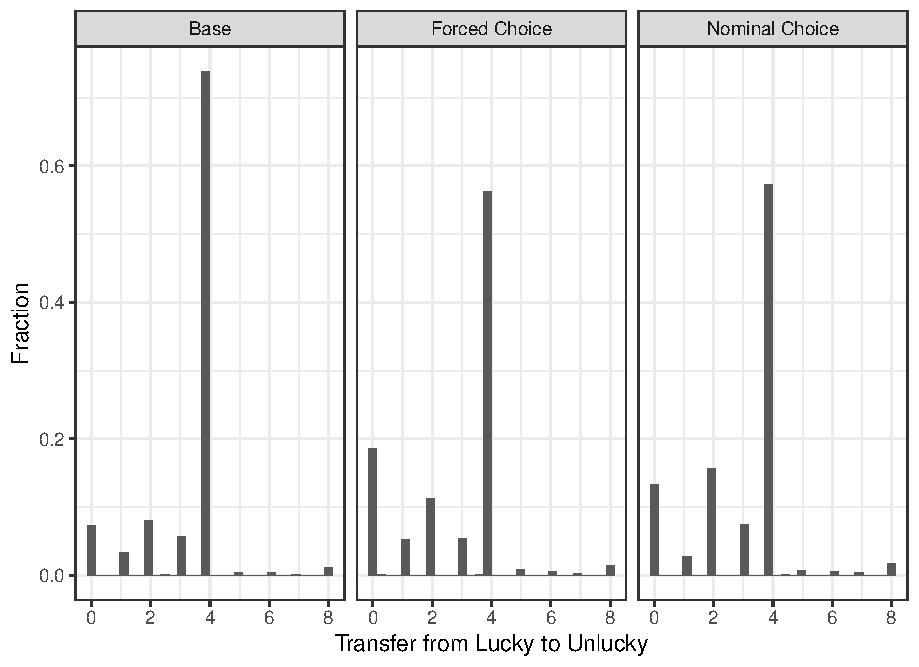
\includegraphics[height=.9\textheight]{../graphs/histograms_kantar.pdf}
	\emph{Note}: The figure shows histograms of the amount of money transferred from the lucky to
	the unlucky participant by the spectator in each treatment. The top two panels are for treatments
	with work requirements, the two bottom panels are for treatments without such a
	requirement.
\end{frame}
%------------------------------------------------------------------------------------

\begin{frame}{Online Experiment Inequality}
	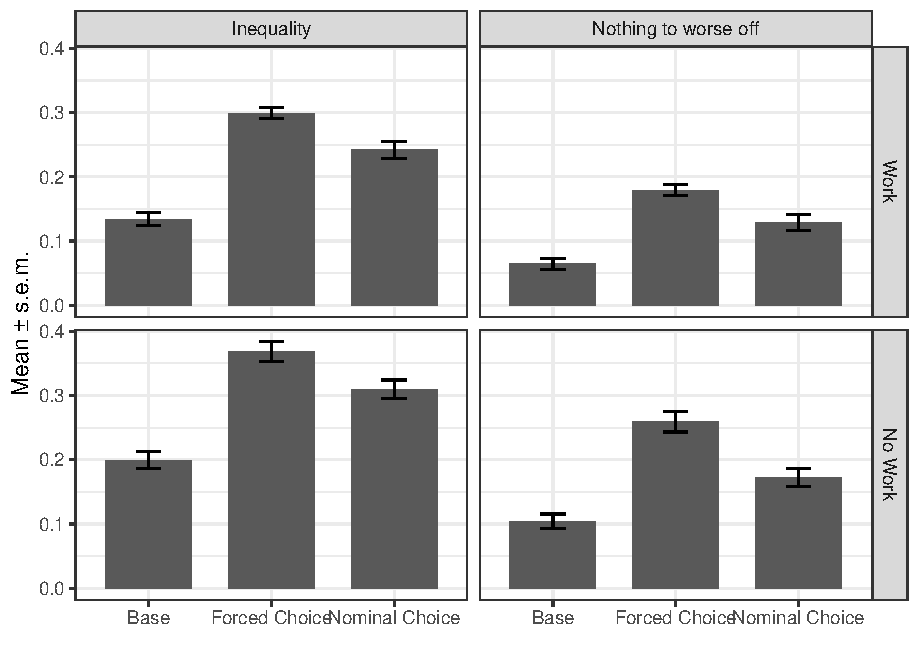
\includegraphics[height=.9\textheight]{../graphs/mean_ineq_nothing_kantar_wd.pdf}
	\emph{Note}: The left panels show the average inequality implemented by the spectators in
each treatment, the right panel shows the share of spectators assigning no income to
one of the participants in the pair in each of the treatments. The top panels show for
treatments with work requirements, the bottom panels show for treatments without
such a requirement. The standard errors of the mean are indicated.
\end{frame}
%------------------------------------------------------------------------------------
%------------------------------------------------------------------------------------
\begin{frame}{Table 3: Online Results -  Regression 1: the role of choice}{\tiny
		%TODO still too long
		% Table created by stargazer v.5.2.3 by Marek Hlavac, Social Policy Institute. E-mail: marek.hlavac at gmail.com
		% Date and time: Fri, Mar 31, 2023 - 18:10:09
		
\begin{table}[!htbp] \centering 
  \caption{} 
  \label{tbl:o1} 
\begin{tabular}{@{\extracolsep{5pt}}lcccccc} 
\\[-1.8ex]\hline 
\hline \\[-1.8ex] 
\\[-1.8ex] & \multicolumn{3}{c}{inequality} & \multicolumn{3}{c}{zero\_to\_worst\_off} \\ 
\\[-1.8ex] & (1) & (2) & (3) & (4) & (5) & (6)\\ 
\hline \\[-1.8ex] 
 treatmentgroupForced Choice & 0.169 & 0.164 & 0.162 & 0.155 & 0.152 & 0.127 \\ 
  & (0.020) & (0.020) & (0.011) & (0.020) & (0.019) & (0.011) \\ 
  & & & & & & \\ 
 treatmentgroupNominal Choice & 0.110 & 0.114 & 0.108 & 0.069 & 0.071 & 0.066 \\ 
  & (0.019) & (0.019) & (0.013) & (0.018) & (0.018) & (0.012) \\ 
  & & & & & & \\ 
 treatmentgroupForced Choice:workp & $-$0.004 & $-$0.004 &  & $-$0.040 & $-$0.040 &  \\ 
  & (0.024) & (0.024) &  & (0.023) & (0.023) &  \\ 
  & & & & & & \\ 
 treatmentgroupNominal Choice:workp & $-$0.003 & $-$0.011 &  & $-$0.004 & $-$0.010 &  \\ 
  & (0.026) & (0.025) &  & (0.024) & (0.024) &  \\ 
  & & & & & & \\ 
 workp & $-$0.065 & $-$0.064 & $-$0.069 & $-$0.040 & $-$0.039 & $-$0.059 \\ 
  & (0.017) & (0.016) & (0.010) & (0.015) & (0.014) & (0.010) \\ 
  & & & & & & \\ 
 leftp &  & $-$0.064 & $-$0.064 &  & $-$0.047 & $-$0.047 \\ 
  &  & (0.011) & (0.011) &  & (0.011) & (0.011) \\ 
  & & & & & & \\ 
 female &  & $-$0.084 & $-$0.084 &  & $-$0.044 & $-$0.044 \\ 
  &  & (0.010) & (0.010) &  & (0.010) & (0.010) \\ 
  & & & & & & \\ 
 age\_h &  & $-$0.078 & $-$0.078 &  & $-$0.057 & $-$0.057 \\ 
  &  & (0.010) & (0.010) &  & (0.009) & (0.009) \\ 
  & & & & & & \\ 
 crt\_h &  & 0.059 & 0.059 &  & 0.052 & 0.051 \\ 
  &  & (0.010) & (0.010) &  & (0.010) & (0.010) \\ 
  & & & & & & \\ 
 university &  & 0.015 & 0.016 &  & 0.021 & 0.021 \\ 
  &  & (0.010) & (0.010) &  & (0.010) & (0.010) \\ 
  & & & & & & \\ 
 high\_income &  & 0.050 & 0.050 &  & 0.049 & 0.049 \\ 
  &  & (0.011) & (0.011) &  & (0.011) & (0.011) \\ 
  & & & & & & \\ 
 Constant & 0.199 & 0.266 & 0.269 & 0.104 & 0.131 & 0.141 \\ 
  & (0.013) & (0.018) & (0.016) & (0.011) & (0.017) & (0.015) \\ 
  & & & & & & \\ 
Joint p-value on work-interactions: & 0.979 & 0.979 &  & 0.157 & 0.144 &  \\ 
Observations & 5,757 & 5,757 & 5,757 & 5,757 & 5,757 & 5,757 \\ 
R$^{2}$ & 0.033 & 0.084 & 0.084 & 0.023 & 0.055 & 0.054 \\ 
\hline \\[-1.8ex] 
\textit{Notes:} & \multicolumn{6}{l}{} \\ 
\end{tabular} 
\end{table}  

	}  % end tiny
\end{frame}

%------------------------------------------------------------------------------------
\begin{frame}{Regression 3}

	\begin{block}{Notes}{\tiny
The table reports linear regressions of the variable “Inequality” (columns (1)–(3),
measuring the inequality implemented by the spectator) and of the indicator variable “Nothing
to the worse off” (columns (4)–(6), taking the value one if the spectator does not assign
any income to one of the participants) on a set of explanatory variables. “Forced
Choice”: indicator variable for the spectator being in the Forced Choice treatment. “Nominal
Choice”: indicator variable for the spectator being in the Nominal Choice treatment.
“Work requirement”: indicator variable for the participants being in a work requirement
treatment. “Left-Wing”: indicator variable for the spectator self-reporting that he or she
voted for a non-right-wing party in the last election. “Female”: indicator variable for the
spectator being female. “Age”: indicator variable for the spectator’s age being at or above
the median in the sample (49 years). “Cognitive Reflection”: indicator variable for the spectator’s
score on the cognitive reflection test being at or above median (2 out of 3 points).
“University education”: indicator variable for the spectator having university education.
“High income”: indicator variable for the spectator having above median income (above
500 000 NOK). Robust standard errors in parentheses.
} % end tiny
	\end{block}
\end{frame}

\begin{frame}{Table 4: Online Results -  Regression 4: Heterogeneous effects on Inequality}{\tiny
		%TODO still too long
		% Table created by stargazer v.5.2.3 by Marek Hlavac, Social Policy Institute. E-mail: marek.hlavac at gmail.com
		% Date and time: Fri, Mar 31, 2023 - 18:10:09
		
\begin{table}[!htbp] \centering 
  \caption{} 
  \label{tbl:o2} 
\begin{tabular}{@{\extracolsep{5pt}}lcccccccc} 
\\[-1.8ex]\hline 
\hline \\[-1.8ex] 
\\[-1.8ex] & \multicolumn{8}{c}{inequality} \\ 
\\[-1.8ex] & (1) & (2) & (3) & (4) & (5) & (6) & (7) & (8)\\ 
\hline \\[-1.8ex] 
 choice & 0.142 & 0.158 & 0.161 & 0.171 & 0.123 & 0.142 & 0.133 & 0.179 \\ 
  & (0.010) & (0.019) & (0.015) & (0.014) & (0.013) & (0.015) & (0.012) & (0.028) \\ 
  & p = 0.000 & p = 0.000 & p = 0.000 & p = 0.000 & p = 0.000 & p = 0.000 & p = 0.000 & p = 0.000 \\ 
  & & & & & & & & \\ 
 choiceTRUE:leftp &  & $-$0.023 &  &  &  &  &  & $-$0.017 \\ 
  &  & (0.022) &  &  &  &  &  & (0.023) \\ 
  &  & p = 0.304 &  &  &  &  &  & p = 0.446 \\ 
  & & & & & & & & \\ 
 choiceTRUE:female &  &  & $-$0.038 &  &  &  &  & $-$0.027 \\ 
  &  &  & (0.020) &  &  &  &  & (0.021) \\ 
  &  &  & p = 0.056 &  &  &  &  & p = 0.196 \\ 
  & & & & & & & & \\ 
 choiceTRUE:age\_h &  &  &  & $-$0.064 &  &  &  & $-$0.061 \\ 
  &  &  &  & (0.020) &  &  &  & (0.020) \\ 
  &  &  &  & p = 0.002 &  &  &  & p = 0.003 \\ 
  & & & & & & & & \\ 
 choiceTRUE:crt\_h &  &  &  &  & 0.043 &  &  & 0.030 \\ 
  &  &  &  &  & (0.020) &  &  & (0.021) \\ 
  &  &  &  &  & p = 0.033 &  &  & p = 0.156 \\ 
  & & & & & & & & \\ 
 choiceTRUE:university &  &  &  &  &  & 0.002 &  & $-$0.006 \\ 
  &  &  &  &  &  & (0.020) &  & (0.021) \\ 
  &  &  &  &  &  & p = 0.936 &  & p = 0.787 \\ 
  & & & & & & & & \\ 
 choiceTRUE:high\_income &  &  &  &  &  &  & 0.028 & 0.018 \\ 
  &  &  &  &  &  &  & (0.022) & (0.024) \\ 
  &  &  &  &  &  &  & p = 0.208 & p = 0.451 \\ 
  & & & & & & & & \\ 
 workp & $-$0.060 & $-$0.060 & $-$0.060 & $-$0.060 & $-$0.060 & $-$0.060 & $-$0.060 & $-$0.060 \\ 
  & (0.010) & (0.010) & (0.010) & (0.010) & (0.010) & (0.010) & (0.010) & (0.010) \\ 
  & p = 0.000 & p = 0.000 & p = 0.000 & p = 0.000 & p = 0.000 & p = 0.000 & p = 0.000 & p = 0.000 \\ 
  & & & & & & & & \\ 
 leftp & $-$0.063 & $-$0.046 & $-$0.064 & $-$0.064 & $-$0.063 & $-$0.063 & $-$0.063 & $-$0.051 \\ 
  & (0.011) & (0.018) & (0.011) & (0.011) & (0.011) & (0.011) & (0.011) & (0.019) \\ 
  & p = 0.000 & p = 0.013 & p = 0.000 & p = 0.000 & p = 0.000 & p = 0.000 & p = 0.000 & p = 0.006 \\ 
  & & & & & & & & \\ 
 crt\_h & 0.059 & 0.059 & 0.059 & 0.058 & 0.026 & 0.059 & 0.059 & 0.037 \\ 
  & (0.010) & (0.010) & (0.010) & (0.010) & (0.017) & (0.010) & (0.010) & (0.017) \\ 
  & p = 0.000 & p = 0.000 & p = 0.000 & p = 0.000 & p = 0.118 & p = 0.000 & p = 0.000 & p = 0.030 \\ 
  & & & & & & & & \\ 
 female & $-$0.084 & $-$0.085 & $-$0.056 & $-$0.085 & $-$0.084 & $-$0.084 & $-$0.084 & $-$0.065 \\ 
  & (0.010) & (0.010) & (0.017) & (0.010) & (0.010) & (0.010) & (0.010) & (0.017) \\ 
  & p = 0.000 & p = 0.000 & p = 0.001 & p = 0.000 & p = 0.000 & p = 0.000 & p = 0.000 & p = 0.001 \\ 
  & & & & & & & & \\ 
 age\_h & $-$0.079 & $-$0.079 & $-$0.079 & $-$0.031 & $-$0.079 & $-$0.079 & $-$0.079 & $-$0.034 \\ 
  & (0.010) & (0.010) & (0.010) & (0.016) & (0.010) & (0.010) & (0.010) & (0.016) \\ 
  & p = 0.000 & p = 0.000 & p = 0.000 & p = 0.054 & p = 0.000 & p = 0.000 & p = 0.000 & p = 0.041 \\ 
  & & & & & & & & \\ 
 university & 0.016 & 0.016 & 0.016 & 0.017 & 0.016 & 0.015 & 0.016 & 0.021 \\ 
  & (0.010) & (0.010) & (0.010) & (0.010) & (0.010) & (0.016) & (0.010) & (0.017) \\ 
  & p = 0.108 & p = 0.109 & p = 0.107 & p = 0.095 & p = 0.110 & p = 0.361 & p = 0.107 & p = 0.210 \\ 
  & & & & & & & & \\ 
 high\_income & 0.050 & 0.050 & 0.049 & 0.049 & 0.050 & 0.050 & 0.029 & 0.035 \\ 
  & (0.011) & (0.011) & (0.011) & (0.011) & (0.011) & (0.011) & (0.019) & (0.019) \\ 
  & p = 0.000 & p = 0.000 & p = 0.000 & p = 0.000 & p = 0.000 & p = 0.000 & p = 0.119 & p = 0.066 \\ 
  & & & & & & & & \\ 
 Constant & 0.264 & 0.253 & 0.251 & 0.244 & 0.279 & 0.265 & 0.271 & 0.239 \\ 
  & (0.016) & (0.020) & (0.018) & (0.018) & (0.017) & (0.018) & (0.017) & (0.024) \\ 
  & p = 0.000 & p = 0.000 & p = 0.000 & p = 0.000 & p = 0.000 & p = 0.000 & p = 0.000 & p = 0.000 \\ 
  & & & & & & & & \\ 
Linear combination &   & 0.135 & 0.123 & 0.107 & 0.166 & 0.143 & 0.161 &  \\ 
 &  & (0.012) & (0.013) & (0.014) & (0.016) & (0.014) & (0.019) &  \\ 
Observations & 5,757 & 5,757 & 5,757 & 5,757 & 5,757 & 5,757 & 5,757 & 5,757 \\ 
R$^{2}$ & 0.081 & 0.081 & 0.082 & 0.082 & 0.082 & 0.081 & 0.081 & 0.083 \\ 
\hline \\[-1.8ex] 
\textit{Notes:} & \multicolumn{8}{l}{} \\ 
\end{tabular} 
\end{table}  

	}  % end tiny
\end{frame}

%------------------------------------------------------------------------------------
\begin{frame}{Online Experiment - Heterogeneous effects on Inequality}

	\begin{block}{Notes}
		The table reports linear regressions of the variable “Inequality” on “Choice”: indicator variable for
		the spectator being in the Nominal Choice or Forced Choice treatment. “Left-wing”: indicator variable for
		the spectator self-reporting that he or she voted for a non-right-wing party in the last election. “Female”:
		indicator variable for the spectator being female. “Age”: indicator variable for the spectator’s age being at
		or above the median in the sample (49 years). “Cognitive Reflection”: indicator variable for the spectator’s
		score on the cognitive reflection test being at or above median (2 out of 3 points). “University education”:
		indicator variable for the spectator having university education. “High income”: indicator variable for the
		spectator having above median income (above 500 000 NOK). “Work requirement”: indicator variable for
		the participants being in a work requirement treatment. Robust standard errors in parentheses. %The full regression table is shown in Table A.2.
	\end{block}
\end{frame}
%------------------------------------------------------------------------------------

	\begin{frame}{Conclusions}

	\begin{block}

		\begin{quote}
			Our findings suggest that people consider the role of choice in determining agency
			and personal responsibility to go beyond the restrictions of the two minimal conditions.
			They find individual choices morally relevant in cases where these choices do
			not change the ex ante probabilities of the outcomes and in cases where there is no
			acceptable alternative to the chosen alternative. Our experimental results thus show
			that the presence of choice is a remarkably powerful source of inequality acceptance
			in society.
		\end{quote}

	\end{block}

\end{frame}


%-----------------------------------------------

	\begin{frame}{Twist}

	\begin{block}

			The authors mention an interaction effect of leftwing votes in the Lab experiment

			I factored the spectators in the Lab experiment age group out of the main online group and looked for 	interactions.


	\end{block}

	\end{frame}



\end{document}
